\documentclass[../Kamil_Kowalewski_Main.tex]{subfiles}

\begin{document} {

    Do eksperymentów został wykorzystany zbiór przedstawiony w~sekcji
    \ref{chapter4:srodowisko_eksperymentalne:zbiory_danych:4}

    \begin{table}[H]
        \scriptsize
        \centering
        \begin{tabularx}{\linewidth}{|L|c|c|c|c|}
            \hline
            % @formatter:off
            Nazwa & Eksperyment \#1 & Eksperyment \#2 & Eksperyment \#3 & Eksperyment \#4 \\ \hline
            Nazwa algorytmu & KMeansEvaluator & FuzzyCMeansEvaluator & BenchmarkEvaluator & BenchmarkEvaluator \\ \hline
            Czas wykonania (s) & 13.266 & 10.189 & 8.907 & 8.469 \\ \hline
            Liczba ofert określona jako wiarygodne & 6 & 6 & 15 & 10 \\ \hline
            Liczba ofert określona jako niewiarogodne & 10 & 10 & 1 & 6 \\ \hline
            % @formatter:on
        \end{tabularx}
        \caption
        [Statystyki dla zbioru danych \#4]
        {Statystyki dla zbioru danych \#4}
    \end{table}

    \begin{figure}[H]
        \centering
        \begin{minipage}[b]{0.49\textwidth}
            \centering
            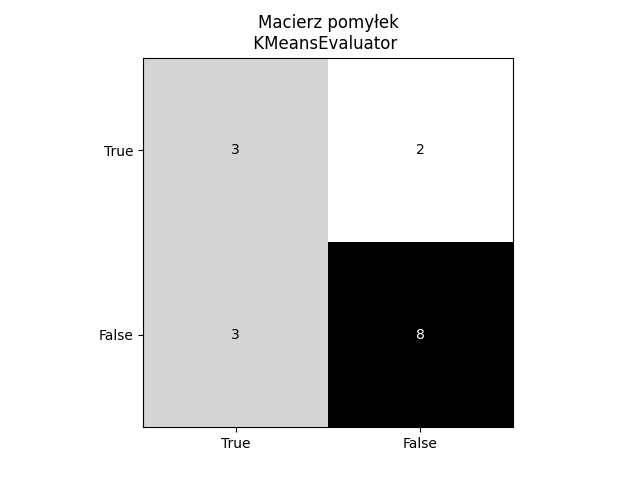
\includegraphics
            [width=\textwidth,keepaspectratio]
            {img/chapter5/dataset4/Logitechm185_KMeansEvaluator.png}
            \caption
            [Macierz pomyłek dla zbioru danych \#4, eksperyment \#1]
            {Macierz pomyłek dla zbioru danych \#4, eksperyment \#1}
            \label{fig:chapter5:eksperymenty:zbior:4:eksperyment:1:macierz}
        \end{minipage}
        \hfill
        \begin{minipage}[b]{0.49\textwidth}
            \centering
            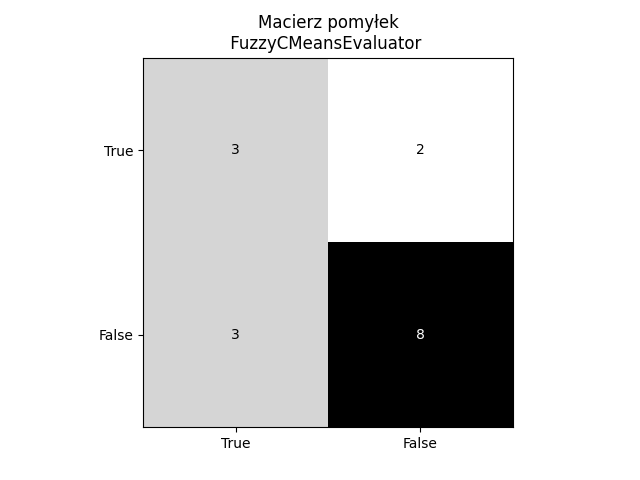
\includegraphics
            [width=\textwidth,keepaspectratio]
            {img/chapter5/dataset4/Logitechm185_FuzzyCMeansEvaluator.png}
            \caption
            [Macierz pomyłek dla zbioru danych \#4, eksperyment \#2]
            {Macierz pomyłek dla zbioru danych \#4, eksperyment \#2}
            \label{fig:chapter5:eksperymenty:zbior:4:eksperyment:2:macierz}
        \end{minipage}
    \end{figure}

    \begin{figure}[H]
        \centering
        \begin{minipage}[b]{0.49\textwidth}
            \centering
            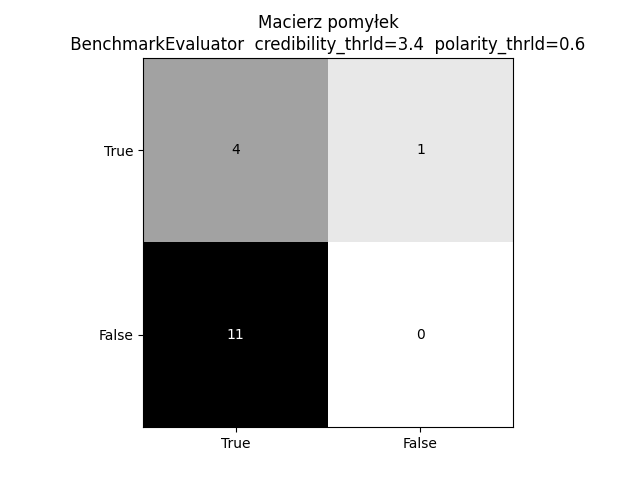
\includegraphics
            [width=\textwidth,keepaspectratio]
            {img/chapter5/dataset4/Logitechm185_BenchmarkEvaluator.png}
            \caption
            [Macierz pomyłek dla zbioru danych \#4, eksperyment \#3]
            {Macierz pomyłek dla zbioru danych \#4, eksperyment \#3}
            \label{fig:chapter5:eksperymenty:zbior:4:eksperyment:3:macierz}
        \end{minipage}
        \hfill
        \begin{minipage}[b]{0.49\textwidth}
            \centering
            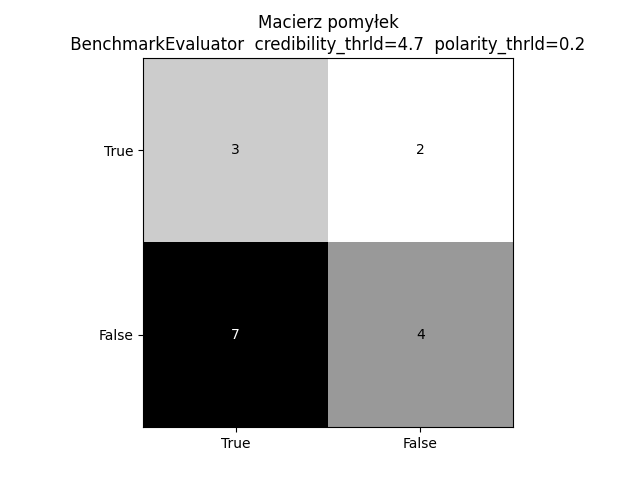
\includegraphics
            [width=\textwidth,keepaspectratio]
            {img/chapter5/dataset4/Logitechm185_BenchmarkEvaluator-1.png}
            \caption
            [Macierz pomyłek dla zbioru danych \#4, eksperyment \#4]
            {Macierz pomyłek dla zbioru danych \#4, eksperyment \#4}
            \label{fig:chapter5:eksperymenty:zbior:4:eksperyment:4:macierz}
        \end{minipage}
    \end{figure}

    \subsection{Podsumowanie uzyskanych wyników}
    \label{chapter5:eksperymenty:zbior:1:podsumowanie} {
        Tak jak w~poprzednich eksperymentach autorska metoda zwraca dla dwóch wariantów
        dokonała takich samych rekomendacji i~popełniła taka samą liczbę błędów. Co
        więcej, występuje analogiczna różnica czasu na korzyść C-Means.

        Metoda literaturowa uzyskała lepsze wyniki dla eksperymentu \#4, gdyż popełniła
        mniej błędów a~dokładnie 2~błędy pierwszego rodzaju oraz 7~błędów drugiego
        rodzaju. W~przypadku eksperymentu \#3 był tylko jeden błąd pierwszego rodzaju
        natomiast było aż 11 błędów drugiego rodzaju. Wynik metody literaturowej nie
        jest akceptowalny natomiast ten uzyskany autorską metodą zawiera błędy, lecz da
        się go zaakceptować.
    }

}
\end{document}
